\chapter{Analiza wyników implementacji kwantowej}
\label{chap:quantum_operations_results}

W niniejszym rozdziale przeprowadzono analizę liczby operacji wykonywanych przez kwantową wersję algorytmu Dijkstry wykorzystującą algorytm wyszukiwania minimum Dürra-Høyera. Analizie poddano te same cztery rodzaje grafów co w pozostałej części pracy: graf rzadki, graf o średniej gęstości, graf gęsty oraz przypadek szczególny.

Liczba operacji wersji kwantowej została wyznaczona zgodnie ze sposobem zliczania opisanym w rozdziale dotyczącym implementacji. Uwzględnia ona koszt przygotowania rejestru w stanie superpozycji oraz liczbę wykonanych iteracji algorytmu Grovera.. Wyniki przedstawiono osobno dla wersji z limitem liczby operacji oraz bez limitu.

\section{Wyniki dla wersji z limitem}

\subsection{Średnia liczba operacji}

\begin{figure}[H]
    \centering
    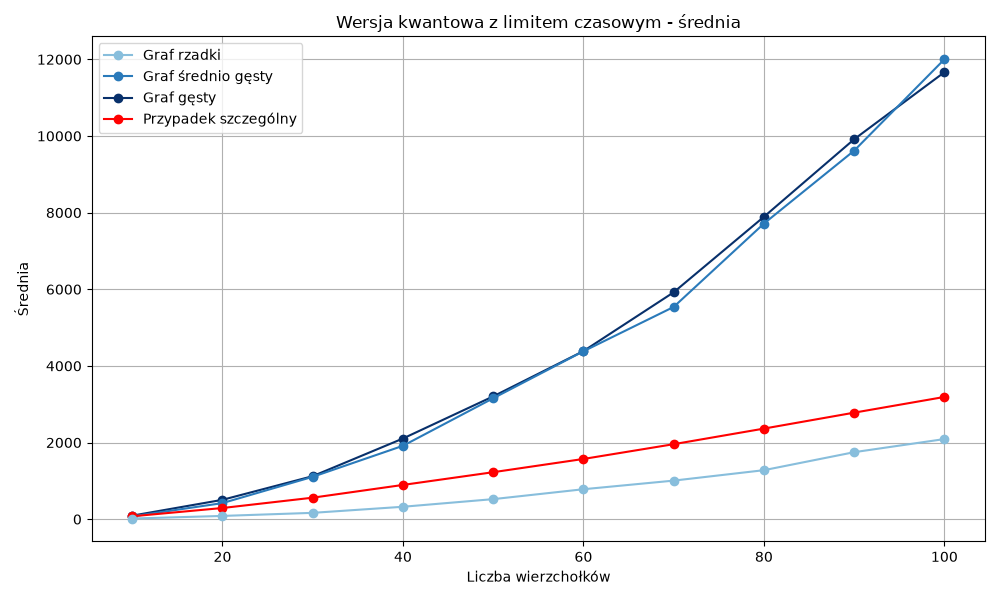
\includegraphics[width=0.95\columnwidth]{images/documentation/quantum/quantum_mean_time_limit.png}
    \caption{Średnia liczba operacji kwantowej wersji algorytmu Dijkstry z limitem liczby operacji.}
    \label{fig:quantum_mean_time_limit}
\end{figure}

Na rys.~\ref{fig:quantum_mean_time_limit} przedstawiono średnią liczbę operacji dla wersji z limitem. Dla wszystkich typów grafów liczba operacji rośnie wraz ze wzrostem liczby wierzchołków. Najmniejszy koszt występuje dla grafu rzadkiego, większe wartości obserwowane są dla przypadku szczególnego, natomiast największą liczbę operacji uzyskują grafy średnio gęste i gęste. Przypadek szczególny, mimo że ma tą samą liczbę krawędzi co graf gęsty, potrzebuje znacznie  mniejszej liczby operacji niż grafy średnio gęste i gęste. Pokazuje to, że koszt kwantowego wyszukiwania minimum w algorytmie Dijkstry zależy nie tylko od liczby krawędzi, ale też od wag krawędzi.

\subsection{Odchylenie standardowe}

\begin{figure}[H]
    \centering
    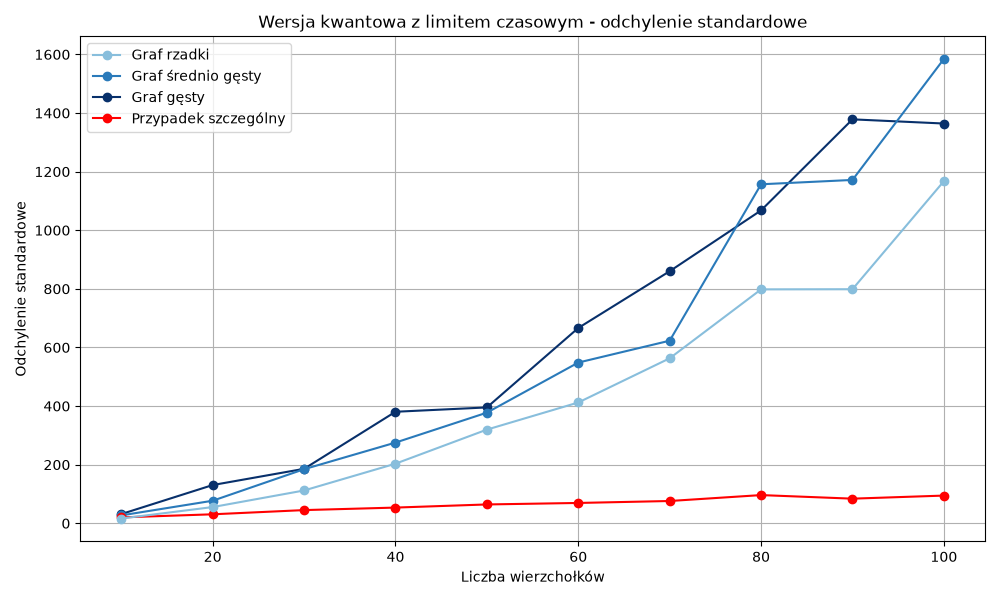
\includegraphics[width=0.95\columnwidth]{images/documentation/quantum/quantum_std_time_limit.png}
    \caption{Odchylenie standardowe liczby operacji kwantowej wersji algorytmu Dijkstry z limitem liczby operacji.}
    \label{fig:quantum_std_time_limit}
\end{figure}

Na rys.~\ref{fig:quantum_std_time_limit} przedstawiono odchylenie standardowe liczby operacji dla wersji z limitem. Wzrost odchylenia standardowego wraz z liczbą wierzchołków wynika z probabilistycznego charakteru algorytmu Dürra-Høyera, w szczególności z losowego wyboru początkowego kandydata na minimum i losowej liczby iteracji wykonywanych w kolejnych próbach BBHT. 

\section{Wyniki dla wersji bez limitu}

\subsection{Średnia liczba operacji}

\begin{figure}[H]
    \centering
    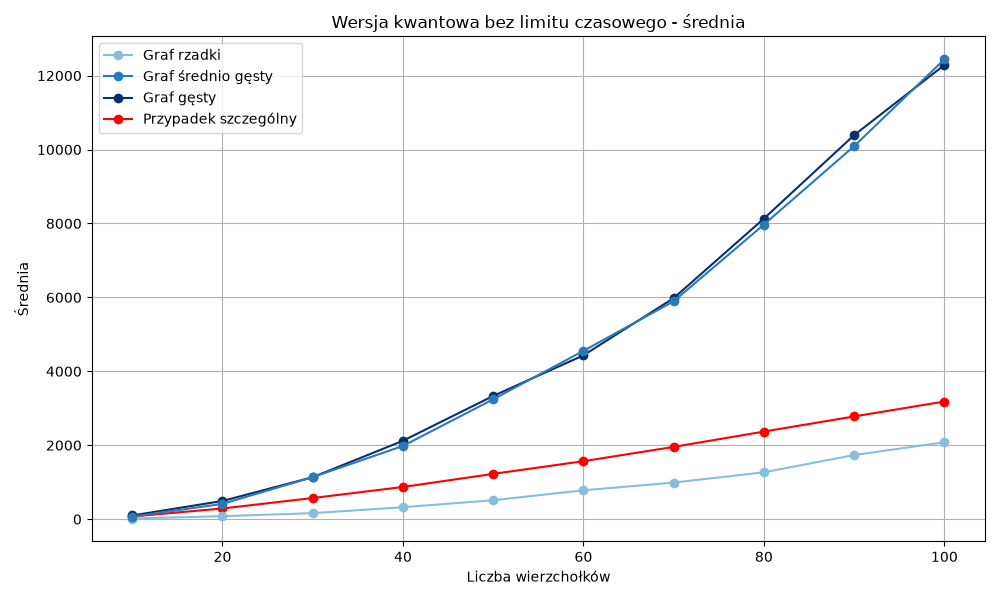
\includegraphics[width=0.95\columnwidth]{images/documentation/quantum/quantum_mean_no_time_limit.png}
    \caption{Średnia liczba operacji kwantowej wersji algorytmu Dijkstry bez limitu liczby operacji.}
    \label{fig:quantum_mean_no_time_limit}
\end{figure}

Na rys.~\ref{fig:quantum_mean_no_time_limit} przedstawiono średnią liczbę operacji dla konfiguracji bez limitu. Dla wszystkich typów grafów liczba operacji rośnie wraz ze wzrostem liczby wierzchołków, a zależności pomiędzy różnymi typami grafów są takie same jak dla wersji z limitem.

\subsection{Odchylenie standardowe}

\begin{figure}[H]
    \centering
    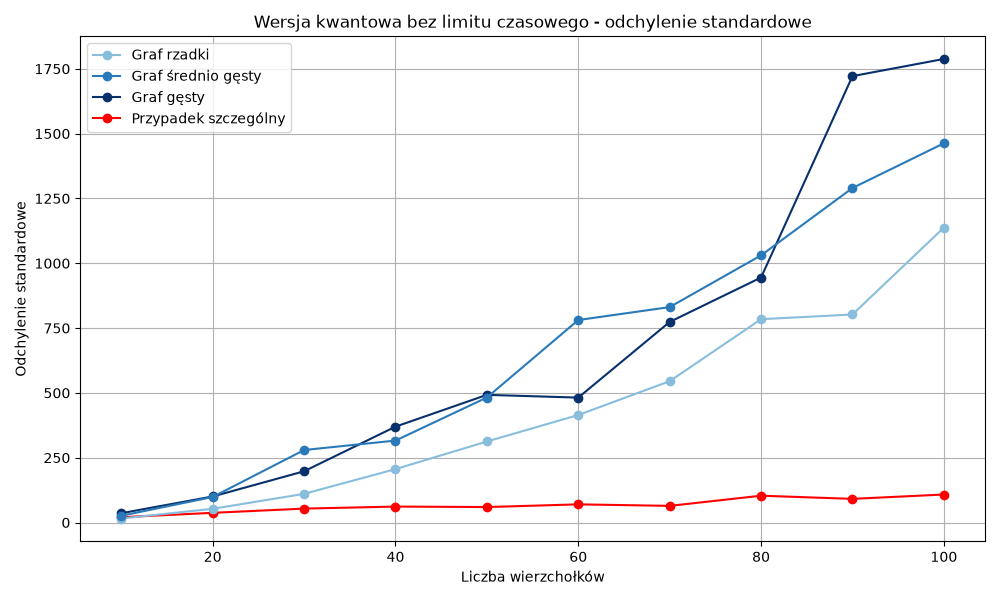
\includegraphics[width=0.95\columnwidth]{images/documentation/quantum/quantum_std_no_time_limit.png}
    \caption{Odchylenie standardowe liczby operacji kwantowej wersji algorytmu Dijkstry bez limitu liczby operacji.}
    \label{fig:quantum_std_no_time_limit}
\end{figure}

Na rys.~\ref{fig:quantum_std_no_time_limit} przedstawiono odchylenie standardowe liczby operacji dla konfiguracji bez limitu. Tutaj podobnie jak dla średniej ogólne tendencje są takie same jak dla wersji z limitem.

\section{Porównanie wersji z limitem i bez limitu}

\subsection{Porównanie średniej liczby operacji}

\begin{figure}[H]
    \centering
    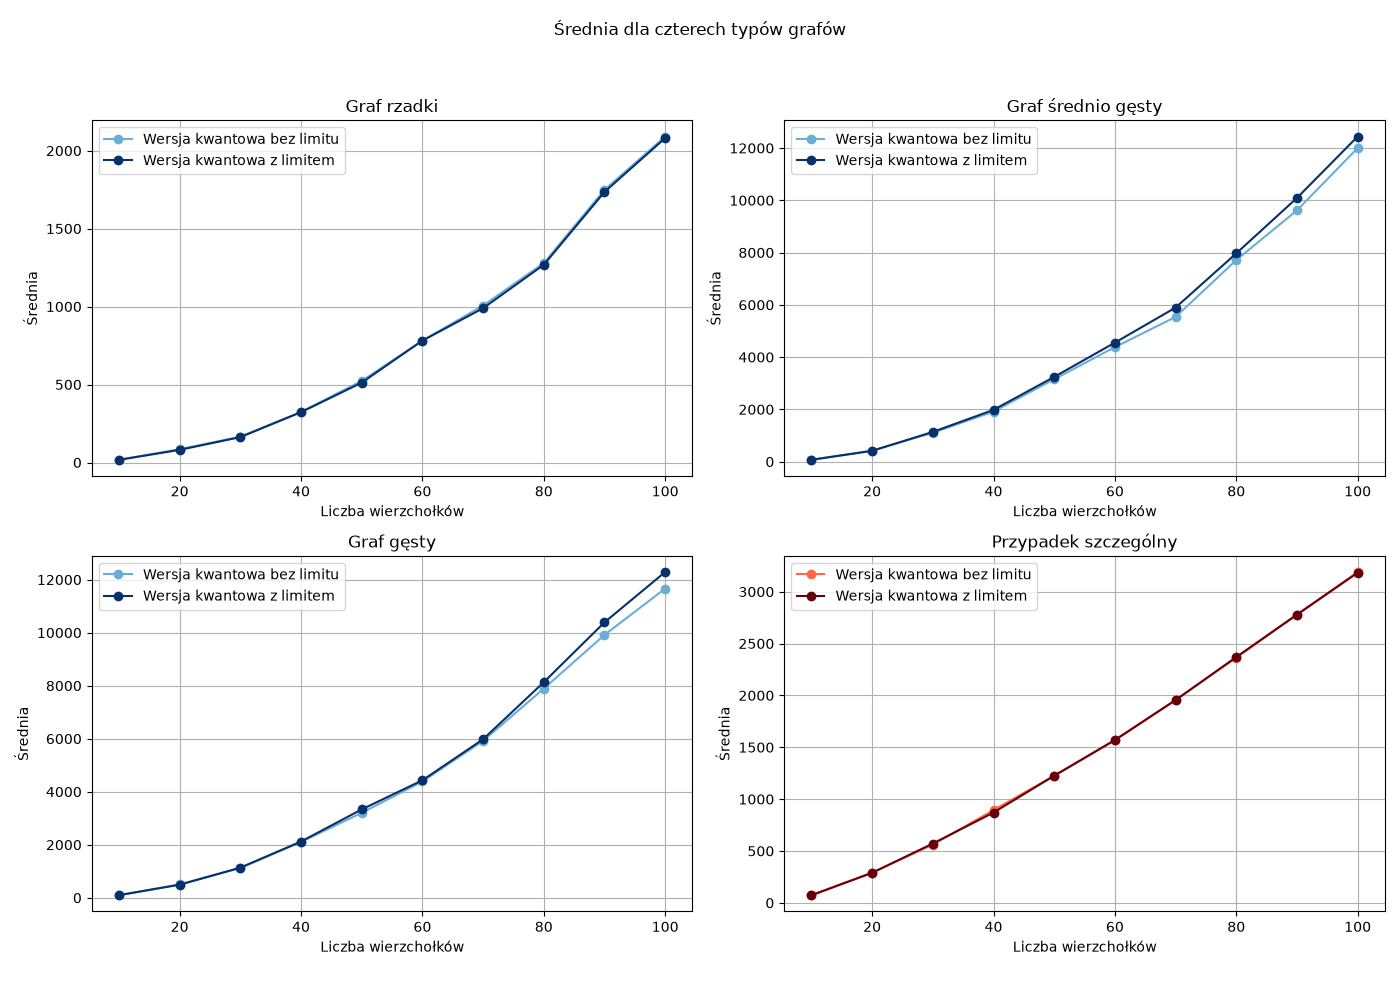
\includegraphics[width=0.95\columnwidth]{images/documentation/quantum/quantum_mean_time_limit_vs_no_time_limit.png}
    \caption{Porównanie średniej liczby operacji wersji kwantowej z limitem i bez limitu dla czterech typów grafów.}
    \label{fig:quantum_mean_time_limit_vs_no_time_limit}
\end{figure}

Porównanie obu wersji przedstawiono na rys.~\ref{fig:quantum_mean_time_limit_vs_no_time_limit}. Dla grafu rzadkiego i przypadku szczególnego wykresy praktycznie się pokrywają dla wszystkich wierzchołków. Dla grafów średnio gęstych i gęstych różnice pomiędzy wersjami stają się bardziej widoczne wraz ze wzrostem liczby wierzchołków. 

\subsection{Porównanie odchylenia standardowego}

\begin{figure}[H]
    \centering
    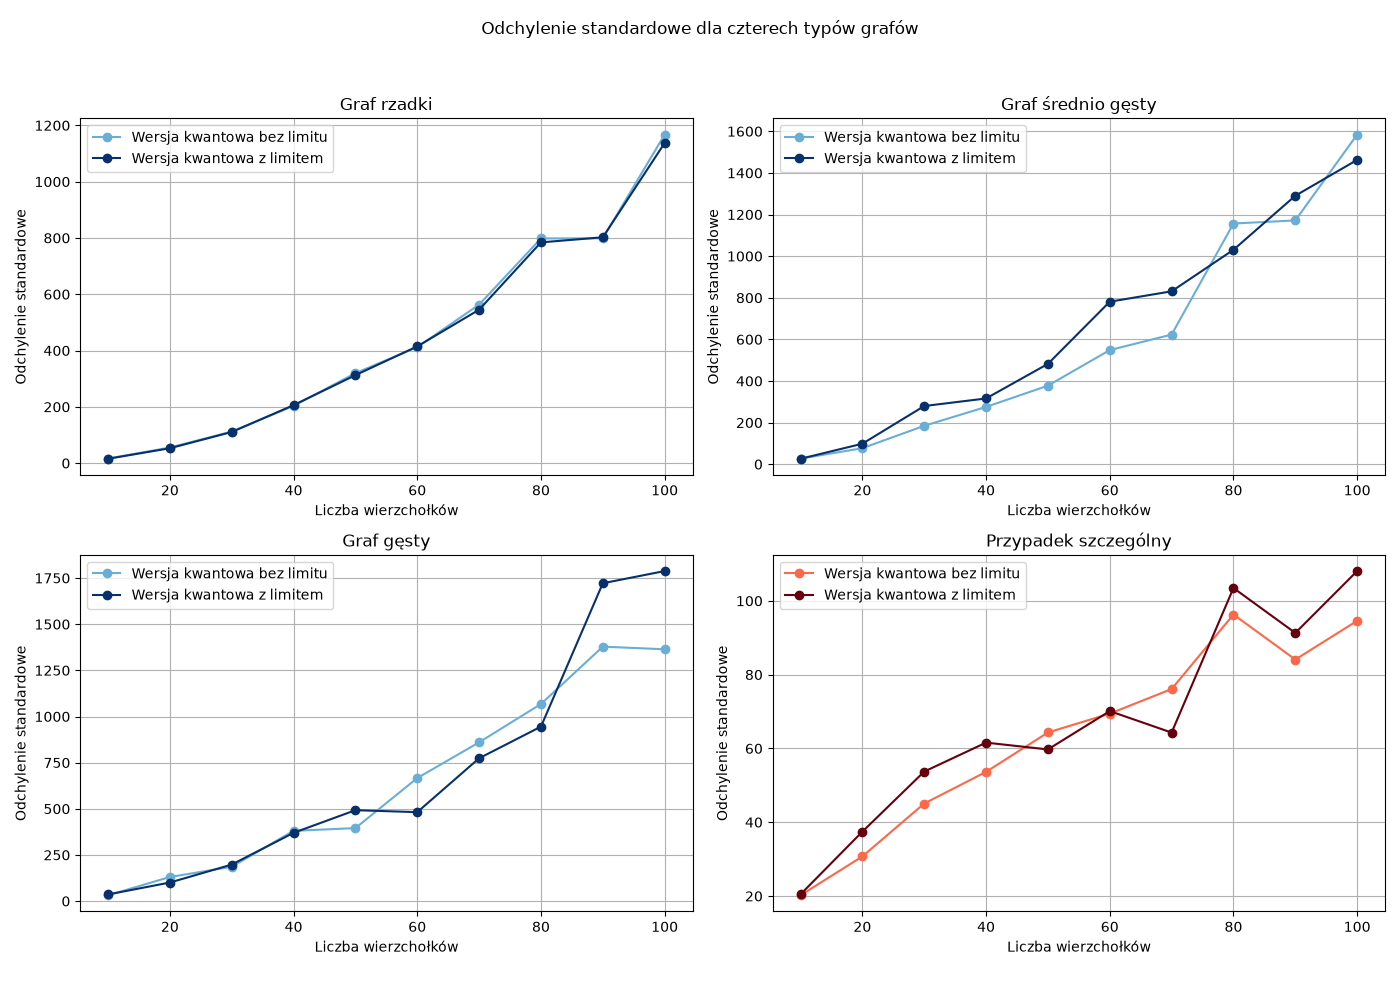
\includegraphics[width=0.95\columnwidth]{images/documentation/quantum/quantum_std_time_limit_vs_no_time_limit.png}
    \caption{Porównanie odchylenia standardowego liczby operacji wersji kwantowej z limitem i bez limitu dla czterech typów grafów.}
    \label{fig:quantum_std_time_limit_vs_no_time_limit}
\end{figure}

Rys.~\ref{fig:quantum_std_time_limit_vs_no_time_limit} umożliwia bezpośrednie porównanie odchylenia standardowego wyników dla obu wersji algorytmu Dijkstry. Dla grafu rzadkiego wartości są niemal identyczne. Większe różnice występują dla przypadku szczególnego oraz grafów średnio gęstych i gęstych.

\subsection{Dlaczego koszt wersji z limitem i bez limitu jest podobny}

Porównując wyniki liczby operacji dla wersji z limitem jak i bez limitu można zauważyć, że są one do siebie bardzo podobne, mimo że w analizie poprawności algorytmu obie wersje zachowują się inaczej. Wersja z limitem dla wielu przypadków zwraca niepoprawny wynik algorytmu Dijkstry, podczas gdy wersja bez limitu jest zawsze poprawna. Wyjaśnić to można, analizując liczbę operacji w zależności od liczby błędnych wyborów minimum.

\begin{figure}[H]
    \centering
    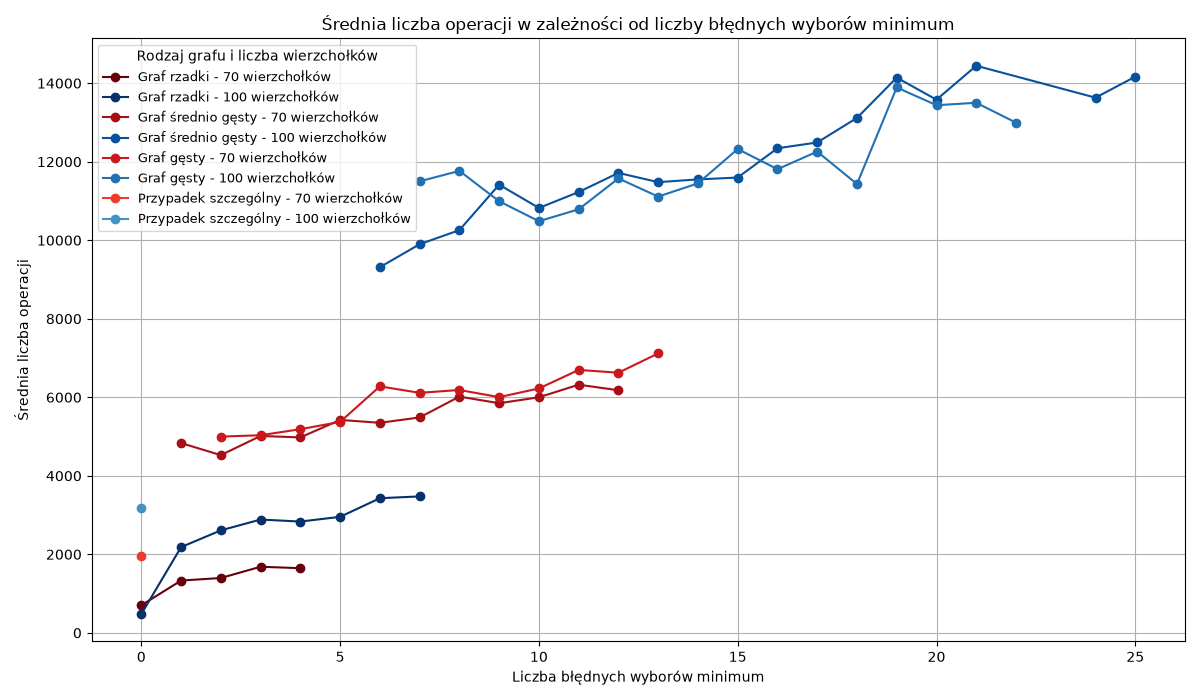
\includegraphics[width=0.95\columnwidth]{images/documentation/quantum/quantum_cost_for_error_minimum.png}
    \caption{Średnia liczba operacji w zależności od liczby błędnych wyborów minimum dla wybranych rodzajów i rozmiarów grafów.}
    \label{fig:quantum_cost_for_error_minimum}
\end{figure}

Na rys.~\ref{fig:quantum_cost_for_error_minimum} przedstawiono zależność pomiędzy liczbą błędnych wyszukiwań minimum a średnią liczbą wykonanych operacji. Dla grafów rzadkich, średnio gęstych oraz gęstych można zaobserwować, że wraz ze wzrostem liczby błędnych wyszukiwań minimum rośnie również średni koszt operacji. Na tej podstawie można stwierdzić, że większej liczbie błędnych wyszukiwań minimum towarzyszy wyższy koszt. Wynika to z faktu, że błędne wyniki wyszukiwania mogą prowadzić do konieczności wykonania kolejnych wyszukiwań, zwiększając liczbę wykonywanych operacji.

Oprócz tego jak przedstawiono w rozdziale~\ref{chap:quantum_probability_results} stosunkowo niewielka część wyszukiwań minimum kończy się niepowodzeniem. Oznacza to, że zarówno w wersji z limitem, jak i bez limitu, głównym czynnikiem wpływającym na średnią liczbę operacji jest koszt poprawnie przeprowadzonych wyszukiwań. W przypadku wersji z limitem niewielka część błędnych wyszukiwań zostaje przerwana po przekroczeniu limitu, co powoduje wykonywanie kolejnych wyszukiwań i w konsekwencji zwiększa ich średni koszt. W wersji bez limitu takie wyszukiwania nie są przerywane, przez co mogą powodować większą liczbę operacji. W rezultacie średnie koszty uzyskane dla obu wersji są podobne.

\section{Zależność pomiędzy kosztem a poprawnością}

Porównanie wyników z analizą poprawności pozwala zauważyć, że ogólnie wprowadzenie limitu nie wpływa pozytywnie na całość algorytmu. Jednak w szczegółach ten wniosek jest zależny od rodzaju rozpatrywanego grafu. Dla grafów rzadkich oraz przypadku szczególnego wprowadzenie limitu nie powoduje znaczących zmian, ponieważ zarówno koszt jak i poprawność jest podobna dla obu wersji. Natomiast dla grafów średnio gęstych i gęstych limit nie powoduje zmniejszenia wykonywanej przez algorytm liczby operacji a tylko znacząco zmniejsza jego skuteczność.
